\chapter{磁聚束系统} \label{ch7}

高速细电子注从电子枪中出来以后便进入互作用区(中间还有一个过渡区)并与螺旋线上传播的高频场发生持续的相互作用,最后在输出端得到放大的高频信号。为了使细电子注能够在细而长的螺旋线中有效地与高频场相互作用,我们必须设法不让电子打到螺旋线上去,使它能顺利地穿过螺旋线,这就是前面所说的如何“维持”电子注的问题。我们知道,螺旋线的长度一般要达到150\textasciitilde 200毫米以上,而直径只有1\textasciitilde 2毫米的细电子注内的电流密度又很大,其空间电荷排斥力也很大在空间电荷排斥力的作用下,细电子注将很快发散变粗,打到螺旋线上去,因而无法穿过细而长的螺旋线与高频场交换能量。另一方面,当我们在输入端送入高频信号时,高频场将沿螺旋线向前传播,并与细电子注相互作用,共同增长。在高频场的同步作用下,细电子注很快地群聚起来。随着群聚的不断增长,群聚电子注内的空间电荷密度也不断增大,其空间电荷排斥力不断增强,这样就在原来发散的基础上增加了一个新的发散力,由于这个发散力是加入高频信号以后才产生的,因此就把它叫做“动态散焦力”。可以看出,动态散焦力实质上也是空间电荷排斥力。

为了使细电子注的直径维持不变,以便有效地与高频场交换能量,我们必须设法在细电子注上面加上一个聚束力,来抵消前面所分析的两种空间电荷排斥力。这个聚束力通常是由外加轴向磁场来产生的,下面将要讲到,轴向磁场对于轴向运动的电子没有作用,但对于径向发散的电子却能够把它们拉回来。这种维持细电子注的方法就称为磁聚束方法,而产生轴向磁场的装置便叫做磁聚束系统。除了磁聚束以外,我们还可以用外加电场的方法来产生聚束力,称为电聚束。磁聚束和电聚束都有好几种方法,本章着重介绍中小功率行波管中最常用的周期永磁聚束法。

怎样才算是一个好的聚束系统呢?

\begin{enumerate}
	\item 聚束系统的好坏主要应当表现在电子注的流通率是不是高?电子注的流通率是指收集极电流$ I_c $占总的阴极电流$ I_K $的百分比。如果阳极电流等于零的话,阴极电流$ I_K $应等于收集极电流$ I_c $和螺旋线电流$ I_H $之和,因此,电子注流通率可以表示为$ \frac{I_c}{I_c + I_H} \times 100\%$,它的物理意义是进入螺旋线的电子注有百分之少能穿过整个螺旋线参予与高频场相互作用的过程。显然我们希望这个百分比越高越好,通常都在90\textasciitilde95\%以上。
	\item 细电子注在螺旋线中流动时应该有良好的稳定性,这样,行波管的工作才能稳定。
	\item 聚束系统的体积要小,重量要轻。这样有利于整个行波管的小型化。
	\item 聚束系统的磁性材料应尽可能做到性能好,来源多,价格便宜,制造工艺简单。
\end{enumerate}

\section{均匀磁场中的电子运动}


磁场对运动着的电子的作用力是克服电子束发散的关键力量。因此,弄清磁场(这里所说的磁场就是磁感应强度)、电子运动速度和磁场加给运动着的电子的作用力这三者之间的关系是很重要的。首先让我们从均匀磁场着手。

如果磁场中任何一点磁感应强度$ B $的大小和方向都完全相同,则该磁场称为均匀磁场。电子在均匀磁场中的运动可以分为三种情况。

第一种情况:带有电荷为$ -e $的电子在垂直于均匀磁场$ B $的平面中以速度$ v $运动。此时,磁场将对运动的电子产生一个作用力$ F $,它的大小等于$ evB $。$ F $的方向则是既和$ B $的方向垂直,又和$ v $的方向垂直,且应服从右手定则,如图\ref{ch7-1}所示。右手定则的意思是:任何电荷$ q $在磁场$ B $中以速度$ v $垂直于$ B $运动时,将受到磁场力$ F $的作用。如果四指从$ v $的方向向$ B $的方向转动,那么拇指的方向就是磁场作用力$ F $的方向。当$ q $是负电荷时$ F $的方向就与拇指的指向相反。由于电子电荷是$ -e $,因此,它受到的作用力$ F $的方向也应当与拇指的指向相反。

\begin{figure}[phtb]
	\centering
	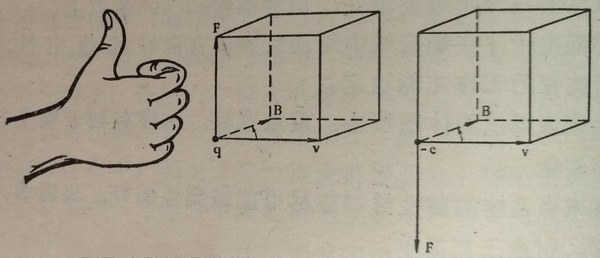
\includegraphics[width=0.8\linewidth]{figure/ch7-1}
	\caption{ 右手定则:四指从$ v $的方向向$ B $转动,拇指方向就是施加在正电荷$ q $上的磁场作用力$ F $的方向,如何电荷为负,$ F $的方向倒转}
	\label{ch7-1}
\end{figure}

在$ F $的作用下,真空中电子的运动将发生什么变化呢?由于$ F $的作用方向垂直于电子运动的方向,因此电子就将在垂直于磁场的平面中作圆周运动,这个情况就象一个人手中拿着条一端系有铁球的铁炼在空中划圈圈那样(图\ref{ch7-2})。人手通过铁练对铁球施一拉力$ F $,这个力就是铁球圆周运动的向心力,它垂直于铁球速度$ v $。同样,磁场力$ F $也是电子圆周运动的向心力,它只改变电子的运动方向而不改变电子运动速度的大小,因而不改变电子的动能。

\begin{figure}[phtb]
	\centering
	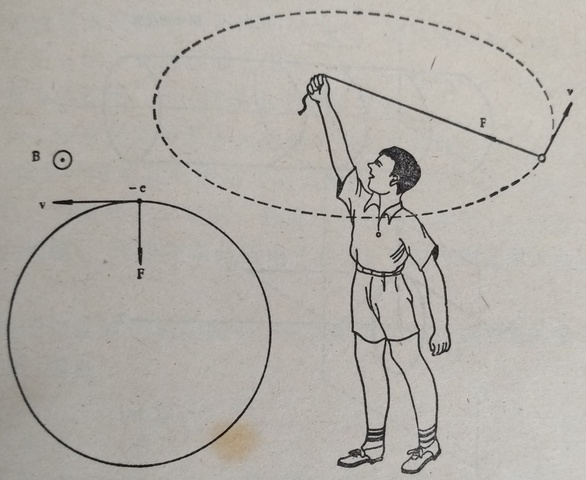
\includegraphics[width=0.75\linewidth]{figure/ch7-2}
	\caption{磁场作用力$ F $垂直于电子运动方向,使电子在垂直于磁场的平面中作圆周运动}
	\label{ch7-2}
\end{figure}

第二种情况是电子速度$ v $的方向与均匀磁场$ B $的方向平行,此时,磁场对电子没有作用。

第三种情况是最一般的情况:电子的运动方向既不和均匀磁场平行又不和均匀磁场垂直(图\ref{ch7-3})。设均匀磁场$ B $的方向是正$ Z $方向,此时我们可以把电子速度$ v $分解成与磁场方向(即$ Z $轴方向)平行的分量$ v_z $以及与磁场方向垂直的分量$ v_{xy} $(即在$ xy $平面内的分量)。磁场对$ v_Z $无作用(因此电子的$ Z $向速度$ v_z $保持不变),但是对$ v_{xy} $将产生作用力$ F_{xy} = e\cdot v_{xy}\cdot B $在$ F_x $的作用下,电子在$ xy $平面内作圆周运动,因此电子的运动就是它在$ Z $轴方向的直线运动和$ xy $平面内的圆周运动的合成,这个合成运动的轨迹是一根螺旋状的曲线,电子好像在一个假想的圆柱面上一边旋转一边沿$ Z $轴向前运动。由此可见,如果有一个本来要离开$ Z $轴向外飞出去的电子,那么,在轴向磁场的作用下,它的运动就将变为沿$ Z $轴作螺旋运动了。这就是说,轴向磁场已经把电子的运动约束在一个圆柱面范围内了。

\begin{figure}[phtb]
	\centering
	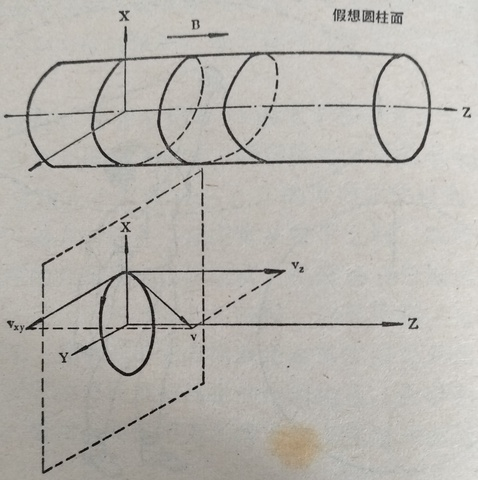
\includegraphics[width=0.6\linewidth]{figure/ch7-3}
	\caption{电子在均匀轴向磁场中作螺旋运动}
	\label{ch7-3}
\end{figure}

把上面的分析用到实际的电子注中去,就能发现磁场对电子注的聚束作用。

我们知道,电子注内的电子受到较强的空间电荷排斥力的作用向外发散,这就说明电子得到了横向速度。如何对付这些发散的电子呢?我们把前面对第三种情况的分析应用于这些发散电子,可见,只要在电子注运动空间加上一个轴向磁场$ B $,就可以使这些发散电子不再向外飞去,而是被约束在假想的圆柱面上沿$ Z $轴作螺旋运动(图\ref{ch7-3})。因此,轴向磁场就起到了聚束的作用,$ F_{XY} $就是电子的聚束力。

为了知道究竞需要多大的轴向磁场才能有效地对电子注聚束,就要弄清楚轴向磁场与电子螺旋运动的关系,例如,电子每打一圈需要多少时间?螺旋运动的半径有多大?等等。为了简化问题,我们先来分析电子在$ xy $平面内作圆周运动的情况。

电子作圆周运动的向心力就是轴向磁场对运动着的电子的作用力,因此,
\begin{equation} \label{eq:ch7-1}
	\frac{mv_{xy}^2}{r} = ev_{xy}B
\end{equation}
式中:$ m $是电子质量,$ r $是圆周运动的半径。由上式可得:
\begin{equation} \label{eq:ch7-2}
	r = \frac{mv_{xy}}{eB}
\end{equation}

圆周运动的周期(即电子飞行一圈所需的时间)为:

\begin{equation} \label{eq:ch7-3}
	T = \frac{2\pi m}{eB}
\end{equation}

这些关系式能不能用到电子的螺旋运动中去呢?我们知道,电子的螺旋运动是轴向(即纵向)直线运动和横向圆周运动的合成。因此,电子的轴向位移将由$ v_z $决定,而横向位移则由$ v_{xy} $和$ B $来决定,也就是说电子的螺旋半径应当等于圆周半径$ r $,螺旋运动的周期应当等于圆周运动的周期$ T $,螺旋运动的螺距$ L $应当等于周期$ T $和轴向速度$ v $的乘积(螺距等于经过一个螺旋周期后电子的轴向位移)。它们的数学表达式分别为:
\begin{equation} \label{eq:ch7-4}
	\begin{aligned}
	r &= \frac{mv_{xy}}{eB}\\
	T &= \frac{2\pi m}{eB}\\
	L &= v_zT = v_z\frac{2\pi m}{eB}
	\end{aligned}
\end{equation}

这是三个基本的关系式,从这三个关系式中我们可以得出几点结论:

\begin{enumerate}
	\item 电子螺旋运动的半径和它的横向速度$ v_{xy} $成正比,和磁感应强度$ B $成反比。因此在一定的磁场下,电子的横向速度越大(发散越严重),螺旋运动的半径就越大。另一方面,磁场越强,电子的螺旋运动半径就越小,也就是旋转的圈圈越由此可见,为了有效地约束发散电子,就应当增强磁场。
	\item 电子的螺旋运动周期仅仅和磁场大小有关,而和电子的速度无关。 \label{item:ch7-1}
	\item 电子螺旋运动的螺距仅仅和磁场大小、电子的轴向速度有关,而和电子的横向速度无关。\label{item:ch7-2}
\end{enumerate}



\begin{figure}[phtb]
	\centering
	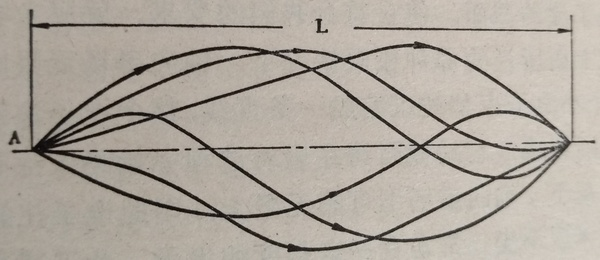
\includegraphics[width=0.6\linewidth]{figure/ch7-4}
	\caption{电子在均匀磁场中会聚示意图}
	\label{ch7-4}
\end{figure}

把上面\ref{item:ch7-1}、\ref{item:ch7-2}两个结论用到实际的电子注中去是很有趣的。我们假定在某一个瞬间有许许多多电子以各不相同的横向速度同时从$ A $点出发向前飞去,它们将在同一个轴向磁场的作用之下,沿$ Z $轴方向作各自的螺旋运动,由于它们的横向速度各不相同,因而螺旋的半径也各不相同。但是它们的螺旋运动周期却是相等的,这就是说它们将同时旋转完一圈,同时开始转第二个圈,同时转完第二圈,这样依次下去。更加有趣的是,由于电子注中的电子都是在同一个加速电压下得到加速的。因此它们的$ Z $向速度$ v $可以认为是相等的,由\ref{eq:ch7-4}式可知,它的螺距$ L $也应该相等。因此,从$ A $点同时出发的许多电子,经过一个周期以后,将同时到达某一点$ A' $,$ A $点和$ A' $点之间的距离等于螺距$ L $,如图\ref{ch7-4}所示。图\ref{ch7-4}再次体现了轴向磁场对发散电子的聚束作用。图中从$ A $点出发的许许多多电子构成了一个很小的电子束,电子束的外径是由横向速度最大的那些电子决定的。因此为了减小电子束的外径就希望增大磁场,使得横向速度最大的那些电子的运动半径在强磁场作用下变得很小,那么横向速度较小的那些电子的运动半径就更小了。图\ref{ch7-5}表示了小电子束截面大小和轴向磁场的关系,在极限情况下,$ B \to \infty $,小电子束被压缩成一条直线。

\begin{figure}[phtb]
	\centering
	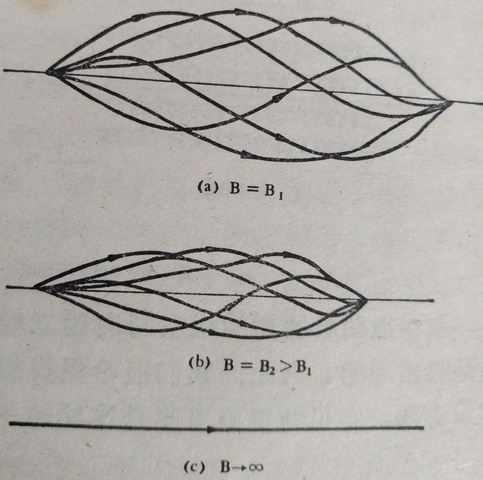
\includegraphics[width=0.55\linewidth]{figure/ch7-5}
	\caption{小电子束截面的直径随轴向磁感应强度的增大而减小}
	\label{ch7-5}
\end{figure}

\begin{figure}[phtb]
	\centering
	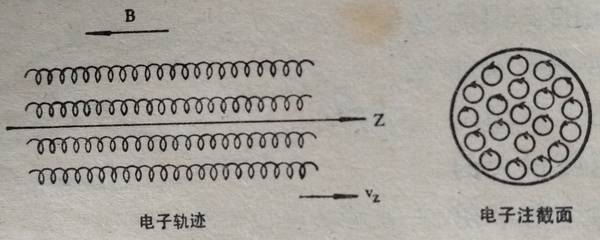
\includegraphics[width=0.65\linewidth]{figure/ch7-6}
	\caption{暴力聚束中的电子轨迹}
	\label{ch7-6}
\end{figure}

实际的电子注截面中存在着许许多多个“$ A $点”,因此,整个电子注可以看成是由许许多多小电子束所组成的。为了减小整个电子注的截面,使它符合我们的要求,就应当增大轴向磁场。在上面所说的那种极限情况下,轴向磁场无限增大,此时,每一个小电子束都被压缩成一条直线,整个电子注就将由无数条直线所组成,它的截面将在运动过程中始终保持不变。但在实际情况下,轴向磁场不可能无限大,因此电子注的截面将不能始终保持不变,常常有一定程度的发散,为了减小这种发散,就必须尽量增大轴向磁场。因此,所需要的磁感应强度是很大的。这种聚束方法叫做暴力聚束或磁限制流聚束。在暴力聚束的电子注中,电子运动的特点是沿着各自的磁力线作螺旋运动即打小圈圈,如图\ref{ch7-6}所示。暴力聚束的最大缺点是所需的磁场要很强,高达几千高斯。

要在细而长的螺旋线空间内建立起高达几千高斯的聚束磁场是很困难的。因此,我们很希望找到一种聚束磁场比较低的聚束方法。布里渊流聚束便是这样的一种聚束方法。

\section{布里渊流聚束}

\subsection{什么叫布里渊流聚束}

我们知道,电子注从电子枪出来尚未射入螺旋线时,由于电子枪内静电场产生的会聚力和电子注内空间电荷发射力相平衡,电子注中的电子便只有轴向速度,没有径向速度。但是电子注射入螺旋线后静电场会聚力便没有了,而空间电荷发射力却依然存在,因此电子注就要发散,它的主要表现是电子注的径向扩张。在发散力作用下,电子有了径向速度。如果我们采用暴力聚束,那么强大的轴向磁场便立刻把电子的径向运动局限在很小的空间内,变成沿磁力线的很小的螺旋运动,在整个电子注中,无数个电子便将围绕着无数根磁力线打着小圈圈前进。

从\ref{eq:ch7-2}式可知,为了使电子打小圈圈前进必须用很强的磁场,这就是暴力聚束需要强磁场的原因。因此我们想,要是能够用打大圈圈的办法来约束电子使它不发散,那么所需的磁场不是可以小得多吗?不过,如果象暴力聚束中那样,电子还是各自绕着各自的磁力线打圈圈,那么圈圈打大了只会使整个截面增大,起不到聚束的作用。我们知道,行波管中的电子注是轴对称电子注,因此,如果能够让所有的电子都绕着共同的轴(即电子注的轴)打圈圈,不也能把它们约束在电子注所占据的范围内吗(图\ref{ch7-7})?而这时由于圈圈要比暴力聚束大得多,因此所需的轴向磁场就可以比暴力聚束时小得多,这的确是一个很好的想法。但是怎样使所有电子都围绕着对称轴打圈圈呢?我们采用了径向磁场的办法。这就是在电子注进入螺旋线时在螺旋线前面利用极靴来得到一个轴对称的径向磁场$ B_r $,极靴是用高导磁率的纯铁制成的,磁力线能够高度的集中到它里面去。由于它的存在,就使轴向磁场的磁力线发生急剧的弯曲,从而产生了轴对称的径向磁场。如图\ref{ch7-8}所示。

\begin{figure}[phtb]
	\centering
	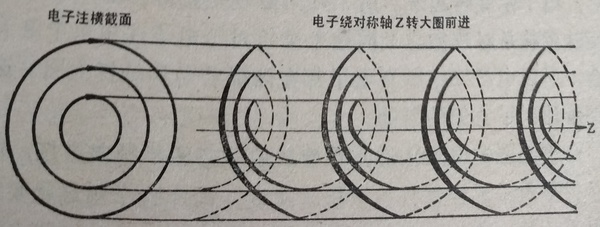
\includegraphics[width=0.85\linewidth]{figure/ch7-7}
	\caption{使电子绕对称轴转大圈以便减小所需要的轴向磁感应强度}
	\label{ch7-7}
\end{figure}

\begin{figure}[phtb]
	\centering
	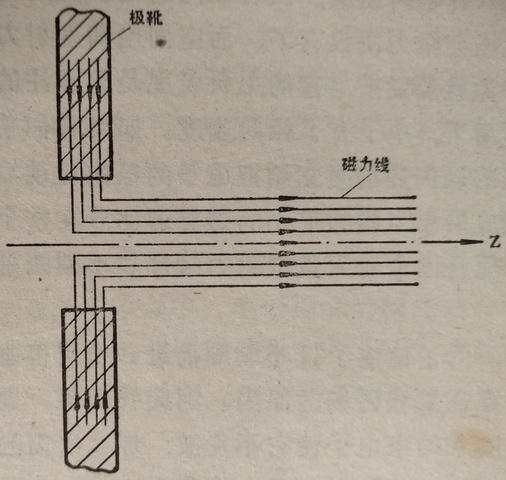
\includegraphics[width=0.65\linewidth]{figure/ch7-8}
	\caption{极靴使磁力线弯曲产生径向磁场}
	\label{ch7-8}
\end{figure}

现在我们来分析一下平行电子注进入图\ref{ch7-8}所示的聚束磁场时的情况。平行电子注首先碰到的是轴对称的径向磁场$ B_r $,在$ B_r $的作用下,根据右手定则,电子受到了切向力$ F_\theta $,因而产生了切向速度$ v_\theta $(我们又称它为旋转速度),有了旋转速度以后,电子便旋转起来。由于径向磁场是轴对称的,因此电子的旋转轴就是对称轴。上面这个分析对于电子注中每个电子都适合,所以电子注中所有电子都在围绕着对称轴打大圈。这样就初步达到了我们的目的。

打着圈圈的电子注进入螺旋线后就碰到了轴向磁场,由于此时每个电子已经都具备了旋转速度。因此这个磁场就要对每个电子作用,产生一个指向对称轴的聚束力,这就是说,电子注进入螺旋线以后,虽然失去了电子枪内的静电场会聚力,但是却由于旋转速度而得了轴向磁场的聚束力,这就给发散力和聚束力的平衡提供了可能。

我们来看看电子注内电子的受力情况。在这种情况下任何一个电子都要受到三种力:(1)空间电荷排斥力$ F_{\textrm{空}} $。半径$ r $处电子所受的空间电荷力$ F_{\textrm{空}} = \frac{eI}{2\pi \varepsilon_0 r \sqrt{2\eta U_0}}$。(2)电子绕对称轴旋转所产生的离心力$ F_{\textrm{离}} $,$ F_{\textrm{离}} = m \cdot \frac{v_\theta^2}{r}$。(3)轴向磁场产生的径向聚束力$ F_{\textrm{聚}} $,$ F_{\textrm{聚}} = ev_\theta B$。这三种力都是径向力。要使电子注的直径保持不变,电子注内各个电子所受到的各种径向力必须平衡,这样才能使电子注维持一定直径。我们考虑电子注边缘其半径为$ r_b $电子的受力情况,为了达到径向力平衡,下列等式必须成立:$ F_{\textrm{聚}}= F_{\textrm{空}} + F_{\textrm{离}}$,即:
$ ev_\theta B \lvert_{r = r_b} = \frac{m v_\theta ^2}{r}\lvert_{r = r_b} + \frac{eI_0}{2\pi\varepsilon_0 r \sqrt{2\eta U_0}} $,经过一些计算,最后可得到:
\begin{equation}   \label{eq:ch7-5}
	B_b = \frac{8.33\times 10^2}{r_b}\cdot \frac{I_0^{1/2}}{U_0^{1/2}}
\end{equation}
式中:$ r_b $:电子注半径,单位为厘米。$ I_0 $:电子注电流,单位为安培。$ U_0 $:电子注电压,单位为伏特。

可见,在这种情况下,为了得到无脉动的电子注,只需要$ B_b $这样大的磁场就行了。后面我们将讲到,聚束磁场太大了反而会引起电子注的脉动。这种聚束方法称之为布里渊流聚束,实现布里渊聚束所需要的磁场值便叫做布里渊磁场值$ B_b $。一般情况下,$ B_b $都在1000高斯以下,因此,比暴力聚束所需磁场要小得多。这一点也可以用“电子打大圈所需磁场要比打小圈时小”来解释。

在实际情况下,由于热初速和阳极孔效应,有一部分电子在进入螺旋线时具有横向速度,不能满足平行入射的要求,因此为了克服这些电子造成的发散,实际所需的磁场值常常为$(1.5\textasciitilde2) B_b $。

\subsection{电子注的脉动}

在实际的聚束系统中,电子注的脉动是难以完全避免的产生脉动的原因主要有:(1)聚束磁场不合适。(2)电子枪和聚束系统对中不良使电子注不能平行入射。(3)聚束磁场的不均匀性。(4)电子注电流本身的起伏。要使这些原因产生的脉动完全消除是极困难的,因此我们所做到的平衡只能是相对的平衡,而不平衡则是绝对的。

下面我们来分析一下单纯因为聚束磁场不合适而引起的电子注脉动。

我们关心的是电子注的直径变化,因此只要观察最外层电子的运动就行了。假定最外层电子以半径$ r_0 $平行入射(图\ref{ch7-9}),由于聚束磁场过强($ B>B_b $),磁聚束力$ F_{\textrm{聚}} $过大,因此使电子产生了向轴的径向速度$ v_r $和径向加速度$ a_r $,电子被拉向轴线,电子注截面就收细了。但是随着电子注截面的收缩,空间电荷的排斥力就要增大,同时$ F_\textrm{聚} $也要随着电子注截面的收细而减小,即聚束力要减小。因而就有可能使$ F_{\textrm{聚}} $和$ F_{\textrm{空}} $、$ F_{\textrm{离}} $达到新的平衡。

\begin{figure}[phtb]
	\centering
	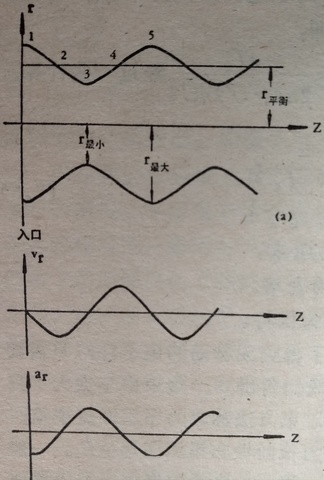
\includegraphics[width=0.45\linewidth]{figure/ch7-9}
	\caption{(a)电子注脉动示意图 (b) $ v_r $和$ a_r $沿$ Z $轴变化情况}
	\label{ch7-9}
\end{figure}


在脉动不大的情况下,最外层电子被拉到平衡半径(图\ref{ch7-9}中“2”点)时,$ F_{\textrm{聚}}$和$ F_{\textrm{空}} $、$ F_{\textrm{离}} $达到新的平衡,因此电子的径向加速度$ a_r=0 $,但此时它的径向速度$ v_r $却达到最大,所以由于惯性,电子还要往里跑,即电子注截面还要继续收缩。在继续收缩的过程中出现了新的不平衡,随着截面的收缩空间电荷发散力进一步增大,而磁场的聚束力却在减小,因此发散力要大于聚束力,出现了把电子往外拉的力,因而产生了离轴向外的径向加速度$ a_r $,电子向轴的径向速度$ v_r $就要减小。到达“3”点时电子的径向速度等于0,但$ F_{\textrm{空}} $达到最大,$ F_{\textrm{聚}} $达到最小,因而电子离轴向外的径向加速度达到最大,电子便要改变运动方向,离开轴线向外扩散。当电子到达“4”点时$ F_{\textrm{聚}} $与$ F_{\textrm{空}} $、$ F_{\textrm{离}} $再次达到平衡,径向加速度$ a_r $等于零,但径向速度$ v_r $达到最大,在惯性作用下电子继续向外运动,此时$ F_{\textrm{聚}} $和$ F_{\textrm{空}} $、$ F_{\textrm{离}} $又开始不平衡,$ F_{\textrm{聚}} $占优势。因而在电子的运动过程中将受到指向轴的径向加速度,电子离轴的径向速度$ v_r $逐渐减小到达“5”点时$ v_r=0 $,$ a_r $最大,电子在$ F_{\textrm{聚}} $的作用下将向内运动。此后的过程又和“1”到“5”点一样,如此反复循环下去。因此,电子注在向前运动的过程中,一会儿收缩一会儿发散,呈现出周期性的脉动。与此同时,电子注还要绕对称轴打圈圈,图\ref{ch7-10}形象地画出了电子注的脉动。

我们常常用脉动的振幅和脉动波长来描述脉动的大小。脉动的振幅是指最外层电子脉动的大小,在小脉动情况下,脉动是围绕着平衡半径进行的,平衡半径就是脉动的平均半径,这时脉动振幅为$ \frac{r_{\textrm{最大}} - r_{\textrm{最小}}}{2} $。脉动波长则是脉动一次前进的距离,如图\ref{ch7-9}中所示。脉动波长与磁场大小成反比,与电子注的加速电压的平方根成正比。

\begin{figure}[phtb]
	\centering
	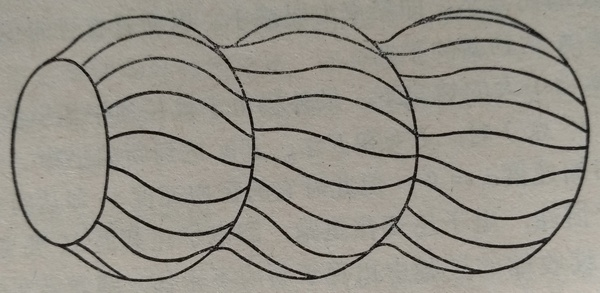
\includegraphics[width=0.5\linewidth]{figure/ch7-10}
	\caption{电子脉动形状示意图}
	\label{ch7-10}
\end{figure}
\section{周期永磁聚束}

布里渊流聚束解决了聚束磁场太大这个问题。接下来就是怎样产生所需要的布里渊磁场了。最初,人们是采用漆包线绕成的多层螺线管线包来产生轴对称磁场的,因而叫做线包聚束(见图\ref{ch7-11})。当线包导线内通以电流时,线包空间内就会产生轴对称磁场,把行波管插到线包的中心,磁场就能对电子注进行聚束。为了得到布里渊流,在电子进入螺旋线的入口处可加一极靴,从而方便地得到轴对称的径向磁场。但是,线包聚束有着很大的缺点:体积大、笨重、效率低。例如,个三厘米波段的小功率行波管,如果用多层线包来产生磁场,那么,线包的重量将达到30公斤,它所消耗的功率将达到400瓦,而行波管本身的重量不过几百克,所消耗的功率不过几瓦或几十瓦。同时,线包的外径也要比行波管大5—10倍。因此,现在已很少采用线包聚束,但这种聚束方法也有一个优点,即它所产生的磁场比较均匀,因此,电子注脉动小,噪声也小。
\begin{figure}[phtb]
	\centering
	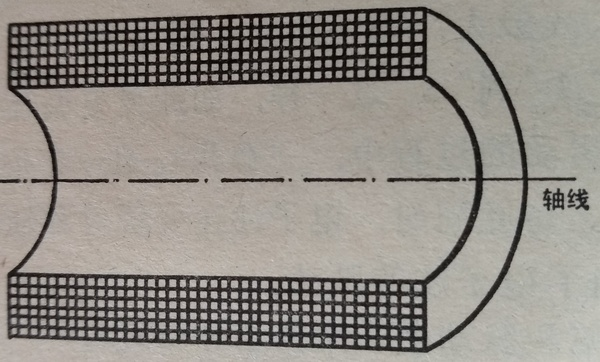
\includegraphics[width=0.47\linewidth]{figure/ch7-11}
	\caption{多层螺旋管线包绕组示意图}
	\label{ch7-11}
\end{figure}

能不能用永久磁铁来产生行波管所需要的轴对称磁场呢?人们曾经尝试过用圆环形永久磁铁(图\ref{ch7-12})来产生轴对称磁场。在磁环厚度不大的情况下,它所产生的轴向磁场沿轴线的分布可以做到比较均匀由于行波管电子注很长,因此也要求圆磁环的轴向长度很长,但是我们发现,随着圆磁环长径比(即磁环的轴向长度与直径之比)的增大,它所产生的磁场的轴向分布将越来越不均匀,这对电子注的聚束带来很大的不利。图\ref{ch7-13}表示了三种长径比情况下磁场的轴向分布。从曲线中可以看出长径比越大,中间跌落得越厉害,磁场越不均匀。
\begin{figure}[phtb]
	\centering
	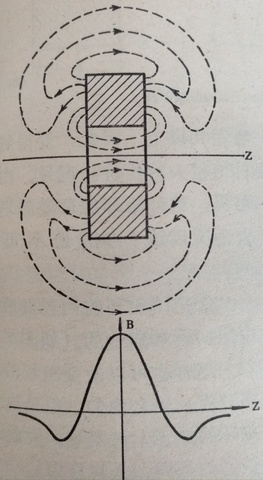
\includegraphics[width=0.35\linewidth]{figure/ch7-12}
	\caption{用环形磁铁产生轴对称轴向磁场}
	\label{ch7-12}
\end{figure}

\begin{figure}[phtb]
	\centering
	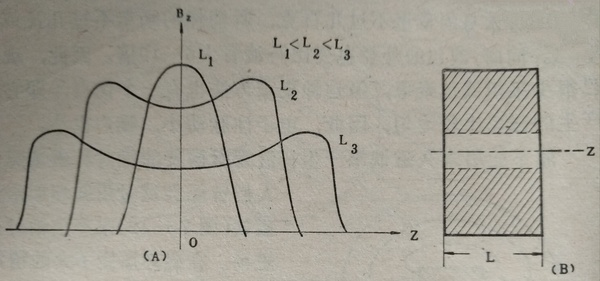
\includegraphics[width=0.65\linewidth]{figure/ch7-13}
	\caption{不同厚度磁环的轴向磁场分布}
	\label{ch7-13}
\end{figure}



为了使磁场的轴向分布尽量均匀,可以有两个办法:

\begin{enumerate}
	\item 增大圆磁环外径。但是这将大大增大磁环的体积和重量,例如,为了使磁场的均匀部分增长一倍,磁环的外径也需要增大一倍,而其体积和重量就将增加到八倍,也就是说,磁环的体积和重量将按长度的三次方成比例地增加。我们知道,行波管轴向长度很长,长径比一般在40以上,因此,要得到如此长的轴向分布均匀的磁场需要付出很大的代价。况且,由图可见,这种磁环的杂散磁场很大,所以这个办法是不可取的。
	\item 把圆磁环的内径做成自中间向两端渐变的(如图\ref{ch7-14})。这样也可以改变磁场的轴向分布,使之均匀。但是这种磁环的加工十分困难,因此这种方法也不可取。我们在实际中采用的是周期永磁聚束。
	\end{enumerate}
\begin{figure}[phtb]
	\centering
	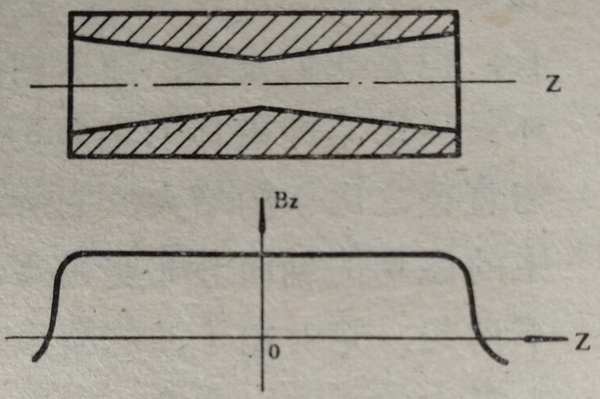
\includegraphics[width=0.4\linewidth]{figure/ch7-14}
	\caption{用磨磁环方法实现均匀轴向磁场}
	\label{ch7-14}
\end{figure}
\subsection{什么叫周期磁场}

我们知道,长径比越大的磁环,其中间跌落也越大。这是什么原因呢?让我们先来做个实验:我们采用多个短磁环重的办法来得到不同长径比的长磁环,并分别画出它们中心磁场的轴向分布,如图\ref{ch7-15}所示。由此可见,单个磁环的磁场轴向分布是脉冲状的,中间有一个主峰,两旁则有两个对称的反峰(为什么产生反峰,见图\ref{ch7-17}。靠外层的磁力线沿$ Z $轴上的方向与磁环中心的磁力线方向相反)。如果我们把两个磁环重迭起来,异极性相对,那么,它们立刻会吸在一起,其合成磁场就应该是两个单磁环磁场之和。因此,合成磁场的轴向分布曲线就可以用两个单磁环的磁场分布曲线达加起来得到。实践证明,这样得到的分布曲线是和实际测得的分布曲线相符合的。可见,磁场中间跌落的原因就在于邻近磁环反峰的抵消作用。同理,我们可以画出由3个、4个以至$ n $个短磁环重选起来构成长磁环的中心磁场分布曲线,并且可以看出:磁环的长径比越大,那么磁场的中心跌落也越严重,举个例子来说,当长径比等于4时磁场就将跌落到原来的60\%。
\begin{figure}[phtb]
	\centering
	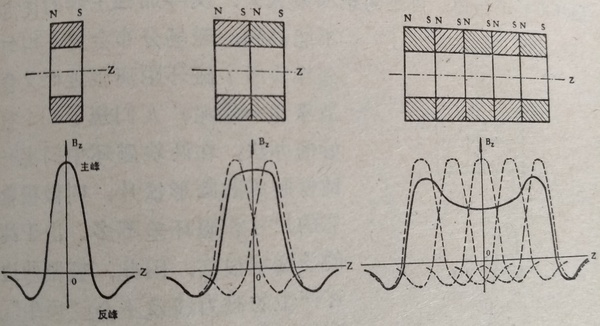
\includegraphics[width=0.65\linewidth]{figure/ch7-15}
	\caption{用短磁环重叠成不同长径比的长磁环}
	\label{ch7-15}
\end{figure}

于是人们就想,如果两个磁环,同极性相对地排列在一起,那么第2块磁环的反峰磁场就不但不会抵消第1块磁环的主峰磁场,而且可以加强第一块磁环的主峰磁场了(见图\ref{ch7-16})。但是要使两块磁环同极性面密合重达在一起是不可能的(斥力太大),只能使两块磁环间有一定的间距,而且这个间距不能太小,否则两个磁环的磁力线要“顶牛”,斥力太大,磁环就容易跑掉。可是间距如果太大,反峰加强主峰的优点就不能得到,磁场分布会更不均匀。怎样使两个磁环距离很近而又稳定地靠在一起呢?人们想了一个很巧妙的办法:在两块磁环中间夹一块纯铁制成的圆形铁片,叫做极靴,它的尺寸和磁环差不多。由于纯铁的导磁率很高,因此,极靴两边磁环产生的磁力线就不会“顶牛”,而且可以很容易地从共用的极靴当中穿过并进入磁环的内部空间,如图\ref{ch7-17}所示,这样,两块磁环就通过极靴紧密地排列在一起了。由于极靴的存在,磁环之间的间距就可以做到很小,例如在1毫米以下。这样就解决了两个磁环之间近距离地稳定地靠在一起的问题。那么极靴会不会使中心磁场减小呢?我们先来看一下单个磁环的情况,实验证明如果在单个磁环两端加上极靴,那么它们的中心磁场不但不会减小而且将得到提高,例如某单个磁环的中心主峰磁场为690高斯,两端加上极靴后就增加到800高斯,即增加了16\%。中心磁场增加的原因可以解释为加了极靴后磁力线向环内集中的结果。现在来看看多个磁环同极性相邻(中间加极靴)地排列在一起的情况,由于相邻磁环反峰和主峰的迭加,中心磁场便得到了加强,但相邻磁环产生的中心磁场是反向的,其轴向磁场$ B_z $的分布如图\ref{ch7-18}所示,可见这是一个周期性的分布,形状接近于正弦曲线,因此被称为周期磁场。周期磁场的峰值要比单个磁环时大很多,例如上例所举的磁环,单环两端加极靴后中心峰值磁场可增加16\%达到800高斯,组成周期磁场后峰值进一步增加到1000高斯,即又增加了25\%,这是很可喜的。在周期场中,为了增加磁场的轴向长度只需要适当增加周期数就可以了,增加的那部分磁场并不会影响原来磁场的轴向分布,整个磁场仍是周期性的。因此,我们不必担心会出现中间跌落的现象,当然也无需用增大磁环直径的办法来改进中间跌落了。相反的,由于磁力线向环内集中(即将无用的环外磁力线集中到环内变为有用),中心磁场反而加强了。而环外的磁力线则很少(相邻磁环产生的环外磁力线相互抵消及磁力线向环内集中两个原因导致),因此周期磁场的漏磁很小,这是它的一个优点。周期磁场的最大优点则是体积小、重量轻。例如,为了使磁场的轴向长度增加到原来长度的$ N $倍,对周期场来说,只要把周期数增加到原来的$ N $倍就可以了,因此其体积和重量都只增加到原来的$ N $倍。但是对均匀场来说,不但磁环的轴向长度要增加,而且磁环的直径也要增加到原来的$ N $倍,因此其重量和体积就要增加到原来的$ N^3 $倍。可见,周期磁场的重量和体积都要比均匀场小$ N^2 $倍,不过实际上一般不到$ N^2 $倍,约为$ N\textasciitilde N^2 $倍。举个例子,某行波管如用均匀场聚束,聚束系统重量需20公斤,但用周期场聚束,聚束系统只需0.5公斤。
\begin{figure}[phtb]
	\centering
	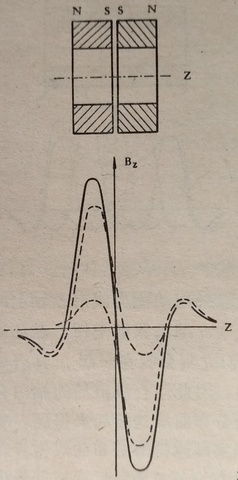
\includegraphics[width=0.37\linewidth]{figure/ch7-16}
	\caption{两块磁环同极性相对地排列在一起,则它们的反峰磁场相互加强相邻磁环的主峰磁场}
	\label{ch7-16}
\end{figure}

\begin{figure}[phtb]
	\centering
	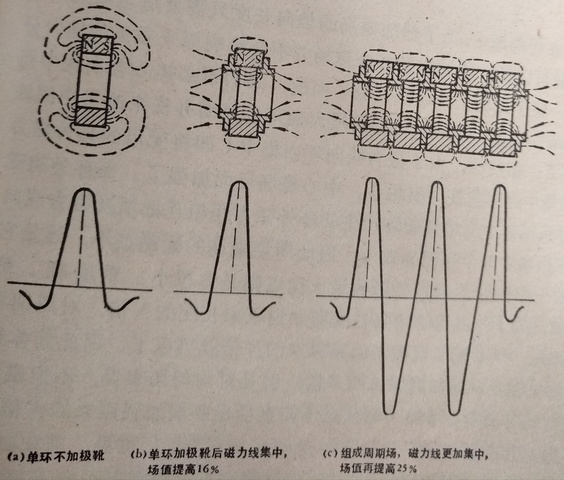
\includegraphics[width=0.65\linewidth]{figure/ch7-17}
	\caption{加极靴后磁力线集中情况}
	\label{ch7-17}
\end{figure}

\begin{figure}[phtb]
	\centering
	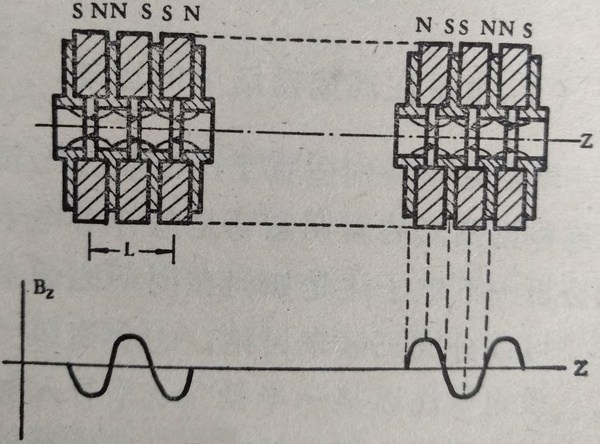
\includegraphics[width=0.5\linewidth]{figure/ch7-18}
	\caption{周期磁场}
	\label{ch7-18}
\end{figure}

\subsection{电子在周期磁场中的运动}


周期磁场特别适宜于产生长径比较大的聚束磁场。为了弄清这种正弦形的周期磁场是怎样对电子注聚束的。下面就让我们分析一下电子注是如何在周期磁场中运动的。


可以分成三区来讨论:(1)会聚区


设电子注以某一半径$ r_{\textrm{最大}} $平行入射到周期磁场中(图\ref{ch7-19}),在磁场入口处轴对称径向磁场的作用下(为了实现布里渊流聚束,在入口处都设置了轴对称的径向磁场),电子得到了较大的旋转速度$ v_\theta $开始绕轴旋转。如果$ r_{\textrm{最大}} $是我们所允许的最大注半径,那么就必须把周期场的峰值轴向磁场放在1-1面处,此时,$ B_z $产生的聚束力$ F_{\textrm{聚}} $就达到最大,同时还应当使$ B_z $足够大,以保证$ F_{\textrm{聚}} >  F_{\textrm{空}} +  F_{\textrm{离}}  $,其中$ F_{\textrm{空}} $是电子注中的空间电荷排斥力,$ F_{\textrm{离}} $是电子绕轴旋转所产生的离心力。


因此,1-1面处作用在电子上的合力就是指向轴的聚束力,且为最大,电子得到了一个径向加速度$ a_r $,并产生了径向速度$ v_r $,因而电子注开始收细。


过了1-1面以后出现了反向的径向磁场($ B_r $变号),电子的$ v_\theta $就要减小,同时$ B_z $也渐渐减小,而随着电子注的收细$ F_{\textrm{空}} $将增大,当电子到达2-2面时将达到$ F_{\textrm{聚}} =  F_{\textrm{空}} +  F_{\textrm{离}}  $(此时电子注的半径等于平衡半径$ r_{\textrm{平衡}} $),因此,电子的径向加速度等于零。
\begin{figure}[phtb]
	\centering
	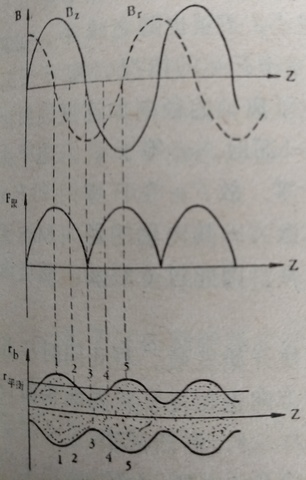
\includegraphics[width=0.37\linewidth]{figure/ch7-19}
	\caption{周期磁场内电子运动分析}
	\label{ch7-19}
\end{figure}

\begin{figure}[phtb]
	\centering
	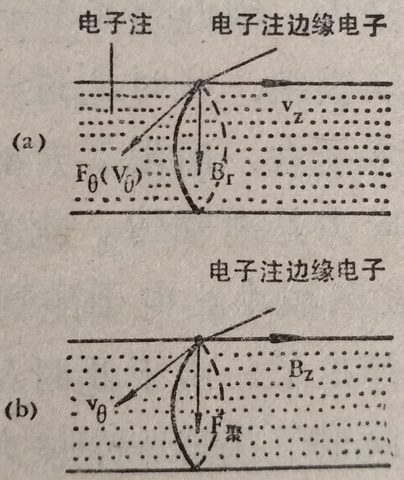
\includegraphics[width=0.25\linewidth]{figure/ch7-20}
	\caption{电子注边缘电子受磁场作用力情况}
	\label{ch7-20}
\end{figure}

(2)由会聚变为发散的过渡区


电子在2-2面处虽然径向加速度等于零,但径向速度$ v_r $却达到了最大,因此过了2-2面以后,在惯性的作用下电子注仍然要继续收细,此时$ B_z $进一步减小,$ F_{\textrm{聚}}$也随之减小,而$ F_{\textrm{空}}$又进一步增大,出现了$ F_{\textrm{聚}} <  F_{\textrm{空}} +  F_{\textrm{离}}  $的情况,电子受到的合成径向力是离轴的。此力产生了离轴的径向加速度因而使电子的$ v_r $逐渐减小。电子注到达3-3面时,$ v_r $等于零,电子注的会聚便停止了。由于此时$ B_z $等于零,故$ F_{\textrm{聚}}$等于零同时$ F_{\textrm{空}}$最大,因而电子获得一个最大的发散力,其离轴的径向加速度最大,另一方面此时$ B_r $最大,$ v_\theta=0 $因此过(3-3)面后电子注将改变旋转方向得到了反向$ v_\theta $。


过了(3-3)面后,电子注便开始发散。与此同时$ B_z $开始向相反方向增大,但是由于$ v_\theta $的方向也相反了,因此仍能得到个向轴的力$ F_{\textrm{聚}}$,此力渐渐增大,$ F_{\textrm{空}}$渐渐减小。


到达(4-4)面时,重新达到$ F_{\textrm{聚}} =  F_{\textrm{空}} +  F_{\textrm{离}}  $。电子的径向加速度$ a_r $等于零,但径向速度$ v_r $最大。


(3)电子注发散逐步减小区域


过了(4-4)面后,虽然由于惯性,电子注仍然要继续向外发散,但此时$ F_{\textrm{聚}}$已占优势,电子就受到了一个指向轴的合力,因此其径向速度慢慢变小。


到达(5-5)面时,电子的径向速度$ v_r $等于零,因而停止向外发散。但此时$ B_z $达到最大,$ B_r=0 $,$ v_\theta $达到最大,因而$ F_{\textrm{聚}}$达到最大。过了(5-5)面后,电子注便逐渐收细,继续重复(1-1)面至(5-5)面的过程。


由上面的分析我们可以看出:

\begin{enumerate}
	\item 周期磁场的峰值对应于电子注最粗的地方,其物理意义就是用最强的磁场聚束力来控制电子注发散最严重的区域。
	\item 会聚力和发散力是交替占优势的,只要磁场选得合适,便可使会聚力做到及时地抵消掉电子注的发散力。
	\item 周期场中的电子注是波浪式前进的,我们称之为“波动”可以看出其“波动”周期等于磁场周期的一半,需要说明的是周期场中的波动和前面讨论过的脉动是两回事,所谓波动是周期场的径向磁场引起的,是周期场所固有的,而脉动则是由于磁场不合适、电子的热初速、阳极孔效应和层流特性等引起的。
\end{enumerate}

这样,我们便对周期场的聚束原理作了一个定性的分析可见,周期磁场是能够很好地完成聚束任务的。


\subsection{电子注在周期场中的脉动}
读者可能要问,周期场中如果磁场不合适,那么会不会电子注产生脉动呢?这是显然的。

从上两节的分析中,我们可以清楚地看到,如果磁场选得合适,便可以使它产生的聚束力在(2-2)面、(4-4)面等处正好等于$ F_{\textrm{空}}$和$ F_{\textrm{离}}$之和,也就是在半个磁场周期内,磁场对电子注的聚束作用正好完全抵消电子注的发散作用。这样对于平行入射的电子注,当它经过半个磁场周期后仍将平行地出来并进入下半个磁场周期,并且在以后的每半个磁场周期中,波动外形维持不变地前进。如果把电子注的各个最粗处(即其顶峰包迹)连起来,则是一条平行于轴的直线。在周期场中,这种情况是最小的脉动情况。


在阴极完全磁屏蔽的情况下,达到最小脉动所需的周期场峰值轴向磁场为
\begin{equation} \label{eq:ch7-6}
	\hat{B_b} = \sqrt{2}B_b = \frac{1.18\times 10^4}{r_b}\frac{I_0^{1/2}}{U_0^{1/2}}
\end{equation}
单位:$ r_b $为毫米,$ I_0 $为安培,$ U_0 $为伏特。


在满足上式的条件下,电子注在轴向磁场峰值处以$ r = r_{\textrm{平衡}} $平行入射,可达到最小的脉动。


实践证明,当$ \hat{B_0}=\sqrt{2} B_b$时,往往不能达到最小的脉动这是因为周期场的最佳聚束条件在实际中常常不能得到满足原因是:(1)高频场和电子注的作用,引起电子注发散。(2)热初速的影响使电子注发散。(3)每个周期中的磁场峰值$ \hat{B_0} $与周期长度不可能完全一致。(4)电子入射半径不可能严格地等于所要求的值,而可能偏高或偏低,还可能会有一定的入射角(即不是平行入射)。(5)周期磁场系统装配不准,磁环的磁性不均匀也会产生干扰。由于这些因素的存在,会不断地破坏脉动的稳定性,如果磁场强一些,那么抵抗干扰的本领也就大一些,因此常常选磁场的磁感应强度峰值$ \hat{B_0} = (1.5\textasciitilde 2)\hat{B_{b}} $。


当$ \hat{B_0} $选择得不合适,或者电子注不是平行入射时,除了周期磁聚束所固有的、周期等于磁场周期一半的波动以外,还存在着周期长得多的脉动。这时波动的顶峰包迹已不再是直线,而是上下起伏的曲线。


现在我们来分析周期场中脉动的形成过程。为讨论方便起见,我们令$ \hat{B_{0b}} = (1.5\textasciitilde 2)\hat{B_{b}} $。下面就来看看$ \hat{B_0} = \hat{B_{0b}} $、$ \hat{B_0} < \hat{B_{0b}} $、$ \hat{B_0} > \hat{B_{0b}} $和$ \hat{B_0} \gg \hat{B_{0b}} $四种情况下电子注的脉动情况。我们把它们画在图\ref{ch7-21}中。
\begin{figure}[phtb]
	\centering
	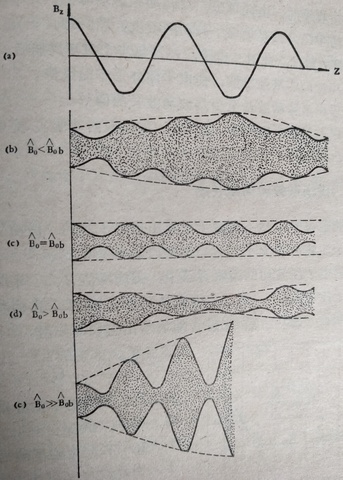
\includegraphics[width=0.6\linewidth]{figure/ch7-21}
	\caption{周期磁场中的电子注的脉动}
	\label{ch7-21}
\end{figure}

图\ref{ch7-21}(a)为周期磁场的磁感应强度分布图。图\ref{ch7-21}(c)为$ \hat{B_0} = \hat{B_{0b}} $时的情况。此时,对于平行入射的电子注来说,只有波动,其顶峰的包迹为一平行于$ Z $轴的直线。图\ref{ch7-21}(b)为$ \hat{B_0} < \hat{B_{0b}} $的情况。开始时,每过半个磁场周期,总的会聚作用小于总的发散作用,所以电子注的半径越来越大当电子注的平均半径大到一定值时,就在该半个磁场周期中总的发散作用与总的会聚作用达到平衡,但这时电子注进入下半个磁场周期时,就不再是平行的,而是有一个向外倾斜的角度,所以电子注的平均半径继续扩大,电子注截面所环链的磁力线增加,会聚力增大,直到总的会聚力大于总的发散力,电子注半径又变小,这样周而复始就形成了脉动。在脉动之上仍迭加有周期磁场聚束所固有的波动。图\ref{ch7-21}(d)是$ \hat{B_0} > \hat{B_{0b}} $的情况。此时也产生脉动,但这时的脉动是以入射半径为顶峰向内收缩的。由此可见,单纯加强磁场峰值,并不能缩小电子注的半径,只是加深了脉动的程度。图\ref{ch7-21}(e)是当$ \hat{B_0} \gg \hat{B_{0b}} $时的情况。此时,电子注经过每半个磁场周期后,不但不会聚,反而严重地发散,使电子注外形不能维持。


一般说来脉动波长至少是波动波长的两倍。


由以上分析可知,$ \hat{B_0} $值只在一定范围内才能实现电子注的聚束,磁场并不是越大越好。


\subsection{磁场系数和周期长度}


周期聚束中既然不可避免地要出现电子注的“波动”,那么,电子注波动的大小究竟和那些因素有关呢?


影响电子注波动的因素有三个:磁场峰值$ \hat{B_0} $,周期长度$ L $和电子注电压$ U_0 $。这三个因素是互相联系的,我们将引入一个新的量一磁场系数$ \alpha $来综合地表示出它们的作用。
\begin{equation} \label{eq:ch7-7}
	\alpha = 2.8\times 10^{-6}\frac{\hat{B_0^2}L^2}{U_0}
\end{equation}

$ \hat{B_0} $,$ L $,$ U_0 $的单位分别为高斯,毫米,伏特。


在阴极完全磁屏蔽的情况下,当$ \hat{B_0}=\hat{B_{0b}}$(对应于最小脉动)时,$ \alpha $对电子注波动的影响示于图\ref{ch7-22}中。由图\ref{ch7-22}可见,$ \alpha $越小,电子注的波动就越小。通常,希望$ \alpha < 0.2 $。

当$ \hat{B_0} \neq \hat{B_{0b}}$时,曲线误差较大,但仍可定性地表示$ \alpha $对电子注波动的影响。


我们把$ a\alpha $关系式中每一项对波动的影响作一些定性解释。

\begin{enumerate}
	\item 如果$ U_0 $和$ L $不变,聚束磁场增强,即$ \hat{B_0} $增大,此时$ \alpha $变大。$ B_0 $增大使$ F_{\textrm{聚}} $比($  F_{\textrm{空}} +  F_{\textrm{离}} $)大得更多,这意味着在图7-19中,电子进入1-1面时受到更大的聚束力,因而有更大的压缩,所以注的波动增大了。
	\item 如果$ U_0 $和$ \hat{B_0} $不变,$ L $增大,此时$ \alpha $也变大。说明电子注在聚束力占优势的区域和发散力占优势的区域停留的时间都增加了,因此电子注的会聚和发散都增强了,波动也就增大了。
	\item 如果$ B $和$ L $不变,当$ U_0 $增加时,$ \alpha $变小。此时电子沿轴运动速度提高,在发散区和会聚区停留时间变短,空间电荷密度也减小了,它的发散力也减小,因此,会聚和发射的程度都要降低,波动变小。
\end{enumerate}


\begin{figure}[phtb]
	\centering
	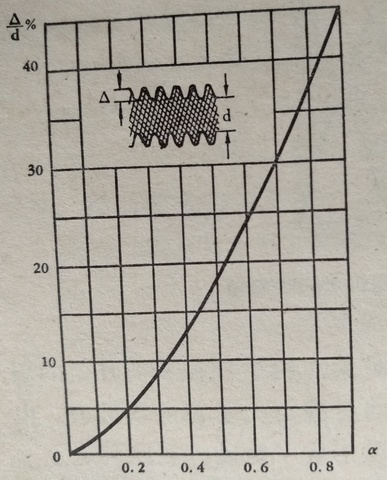
\includegraphics[width=0.37\linewidth]{figure/ch7-22}
	\caption{阴极完全屏蔽下,$ \hat{B_0} = \hat{B_{0b}} $时,磁场系数$ a $与电子注波动$ \frac{\Delta}{d} $的关系}
	\label{ch7-22}
\end{figure}
从图\ref{ch7-22}可以看出,$ \alpha $这个参量对于电子注的波动有很大的影响,为了不影响高频性能我们希望控制电子注的波动在10\%以下,因此就要求$ \alpha < 0.2 $。通常在设计中,$ U_0 $和$ \hat{B_{0}} $是先定的,故$ \alpha $的大小主要由$ L $来决定。$ L $小,波动程度就小,对电子注与高频场作用有利。但是,此时磁环厚度也减小了,为了获得同样的$ \hat{B_0} $就要增大磁环的外径,这样,聚束系统的体积和重量都要增大。此外,$ L $小了还会给输能装置的安装带来困难,因此$ L $太小对我们是不利的。我们必须兼顾各方面的要求来选择一个适中的$ L $值。
\subsection{怎样决定磁环的尺寸?}
也就是如何设计一个周期磁聚束系统的问题。我们不准备作详细的介绍,仅仅简单的提几个原则,目的是使读者对于实际的周期聚束系统有一个尺寸方面的印象。

\begin{figure}[phtb]
	\centering
	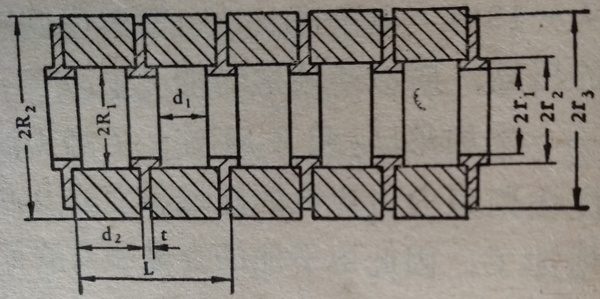
\includegraphics[width=0.5\linewidth]{figure/ch7-23}
	\caption{周期磁场的结构参量}
	\label{ch7-23}
\end{figure}
我们把周期场的尺寸画在图\ref{ch7-23}中,图中符号说明如下:


$ r_1 $:极靴环内半径

$ r_2 $:极靴环外半径

$ r_s $:极靴片外半径

$ R_1 $:磁环内半径

$ R_2 $:磁环外半径

$ d_1 $:极靴间隙

$ t $:极靴片厚度

$ d_2 $:磁环厚度

$ L $:磁场周期


首先介绍一下我们所用的永磁材料,对永磁材料的要求一般是:矫顽力$ H_c $高,最大磁能积$ (B\cdot H)_\textrm{max} $大,剩磁$ B_r $大,温度系数小。简单说来,矫顽力表示了磁铁(即永磁材料)抵抗去磁的能力;剩磁表示了磁铁的磁化程度;而磁能积的意义则是:当磁铁体积一定时,磁能积越大,则磁铁给外界空间的磁能就越多;当磁铁给外界空间的磁能一定时,磁能积越大则所需磁铁体积越小。

我们知道,在周期场中,磁环是互相排斥地排列的,受到很强的去磁场作用,因此,在保证一定的磁能积的前提下,我们总是希望矫顽力尽可能高些。

常用的永磁材料有两大类:钡或锶铁氧体和磁钢。

铁氧体又可分为同性铁氧体和异性铁氧体两种。

同性铁氧体是干粉压制而成。压时外面不加充磁磁场,压完焙烧后各个方向磁性能一样,充磁后能达到的指标较低:矫顽力$ H_c = 1900\textasciitilde 2000 $奥斯特,最大磁能积$ (B\cdot H)_\textrm{max} = 0.95\times 10^6 \textasciitilde 1.2\times 10^6$奥高,剩磁$ B_r = 2000\textasciitilde 2100 $高斯。同性铁氧体的优点是压制容易,磁性能另散小,同一磁环中磁性均匀磁性能稳定,机械加工(研磨)时不易破裂。

异性铁氧体是湿压而成,利用钡或锶铁氧体微粒磁化性能上的各向异性,加压成型时在将来要充磁的方向上加磁场,使微粒最大磁化方向转到磁场方向。焙烧后各个方向磁化能力很不一样,只有沿压力方向充磁才能充上最大的磁性。充磁后可以得到较高的磁性能:$ H_c = 2500\textasciitilde 3000 $奥,$ (B\cdot H)_\textrm{max} = 3\times 10^6 \textasciitilde 3.7\times 10^6$奥高,$ B_r = 3000\textasciitilde 4000 $高。

总的说来,铁氧体的优点是矫顽力大,去磁曲线的线性好,价格便宜。但其主要缺点是温度系数大,约为$ -0.2 \%/\si{\degreeCelsius}$。此外,它的磁性能均匀性也较差。由于温度系数比较大,因此它只能工作在$ -20\si{\degreeCelsius}~\textasciitilde +40\si{\degreeCelsius} $范围内,增加温度补偿后可扩大到$ -40\si{\degreeCelsius}~\textasciitilde +50\si{\degreeCelsius} $。

磁钢是钻的合金,最常用的是铝镍钴合金,因成份和磁性能的不同而有多种牌号。我们在行波管中用得最多的是铝镍钴8(AlNiC0-\uppercase\expandafter{\romannumeral8}),其磁性能为$ H_c = 1500\textasciitilde 1800 $奥,$ (BH)_\textrm{max} = (5\textasciitilde 5.5)\times 10^6$奥·高,$ B_r = 8000\textasciitilde 9000 $高斯。还有一种铝镍钴5,它的$ B_r $高达12000高斯,但是$ H_c $仅800奥,主要用于“M型”器件中。铝镍钴磁钢的突出优点是温度系数很低,仅$ -0.04 \%/\si{\degreeCelsius}$,因此工作非常稳定(在$ -65\si{\degreeCelsius}~\textasciitilde +100\si{\degreeCelsius} $范围内可稳定地工作)。此外它的磁能积也较大。它的缺点是矫顽力较小,去磁曲线线性较差,价格较贵。


近年来,研制出一种新型钻合金,叫钴磁钢,它的磁性能非常好:$ H_c $达9000奥,$ (BH)_\textrm{max}$达$(15\textasciitilde 20)\times 10^6$达(15~20)×10奥高,$ B_r $为9000高,去磁曲线的线性也较好。由于它的磁性能比铝镍钴8高得多,因此,利用它作为周期聚束系统的永磁材料可以大大减小聚束系统的体积和重量。例如,利用钐钴磁钢后,可以将原来90公斤重的聚束系统减轻到只有3公斤。钐钴磁钢的主要缺点是价格较贵,但近年来经过努力已大大降低,因此这种磁钢有着很好的发展前景。


通常,我们是根据电子注的电压$ U_0 $,电子注电流$ I_0 $和束半径$ r_b $来设计周期聚束系统的。它的步骤是:
\begin{enumerate}
	\item 选择磁场的峰值$ \hat{B_{0}} $,一般是$ (1.5\textasciitilde2) \hat{B_b}$ ;
	\begin{equation*}
		\hat{B_0} = (1.5\textasciitilde2) \frac{1.18\times10^4}{r_b}\cdot\frac{\sqrt{I_0}}{\sqrt{U_0}}\,\textrm{高斯}
	\end{equation*}式中:$ I_0 $:安,$ U_0 $:伏,$ r_b $:毫米。
	\item 选择磁环材料;
	\item 确定周期$ L $:可根据$ \alpha < 0.2 $的原则来选择。
	\begin{equation*}
		\alpha = 2.8\times 10^{-6}\frac{\hat{B_0^2}L^2}{U_0}
	\end{equation*}
	式中:$ \hat{B_0} $:高斯,$ L $:毫米,$ U_0 $:伏特。$ L $选得较大磁场值可以较高,因而达到同样大小的$ \hat{B_{0}} $所需的体积和重量就可以比较小,但$ L $大,电子注的波动也大,因此要兼顾各方面来选择$ L $。
	\item 极靴内半径$ r_1 $:尽可能小,可使磁聚束系统重量减轻。般等于管壳的外半径。
	\item 极靴间隙$ d_1 $:取$ d_1/L=0.2\textasciitilde0.25 $。在$ L $确定后,如果$ d_1 $减小,则$ \hat{B_0} $可增大。理论上$ \frac{d_1}{L} = \frac{1}{3}$时,轴上磁场分布最接近正弦,电子注波动小。但此时$ \hat{B_0} $较低,所以通常选取$ \frac{d_1}{L} $在$ 0.2\textasciitilde0.25 $间。
	\item 磁环厚度$ d_2 $:选择的原则是在极靴不饱和的前提下尽可能使$ d_2 $大些,这样就可以得到高的$ \hat{B_0} $值。一般选$ \frac{d_2}{L} =0.4\textasciitilde0.5$左右。由于极靴片的厚度$t=\frac{L}{2}-d_2$,有时为了使极靴不饱和我们先选择$ t=0.1L $,算出$ L $后由$ t $再来决定$ d_2 $,也是一样的。
	\item 磁环内半径$ R_1 $:一般我们采用内对中结构,即靠极靴内半径和管壳滑配合来保证对中,然后磁环内半径再和极靴端部滑配。因此,磁环内半径$ R_1 $和极靴环外半径$ r_2 $是相等的。我们选择$ r_2 $时常使环厚$ (r_2 - r_1) $略比极靴片之半大些即可,一般选择为$ 0.7t $,因此,$ R_1=r_2=r_1+0.7t $。
	\item 根据曲线可查得$ R_2 $值。一般极靴片的外径$ r_3 $和$ R_2 $相等或稍小于$ R_2 $。
	\item 根据螺旋线总长算出周期数。
\end{enumerate}
这样,一个周期磁聚束系统就计算完毕了。

下面我们结合一个实例来说明周期场的计算。

某行波管电子注电压$ U_0=2500 $伏,电子注电流$ I_0=40 $毫安,电子注半径$ r_b=1.23 $毫米,管壳外半径为3.1毫米,金属陶瓷结构。

\begin{enumerate}
	\item 计算聚束所需的轴向峰值磁场$ \hat{B_0} $。
	\begin{equation*}
	\hat{B_0}=\frac{1.18\times10^4}{r_b}\cdot\frac{{I_0}^{1/2}}{{U_0}^{1/2}}
	\end{equation*}将已知值代入可算得$ \hat{B_b}=538 $高斯。
	
	为了得到可靠的聚束,应选取$ \hat{B_0}=(1.5\textasciitilde2)\hat{B_b} $。,我们取$ \hat{B_0} = 1.5\hat{B_b}=1.5\times538=800 $高斯。
	\item 选择材料。
	
	因为$ \hat{B_0}=800 $高斯是不算很强的磁场,故决定选择铝镍钴8作为磁性材料,其稳定性好。
	\item 确定周期L。
	
\begin{equation*}
		\begin{aligned}
	\textrm{由}\quad \alpha &= 2.8\times10^{-6}\frac{\hat{B_0^2}L^2}{U_0} < 0.2\,\textrm{可得:}\\ L &< 270\frac{\sqrt{U_0}}{\hat{B_0}}
		\end{aligned}
\end{equation*}将$ U_0 $、$ \hat{B_0} $代入即得到$ L < 16.8$毫米。我们选择$L = 12 $毫米。
	\item 确定$ r_1 $。
	
	因为是金属陶瓷结构,故极靴可与金属管壳滑配,因此取$ r_1=3.1 $毫米。
	\item 确定$ d_1 $。
	
	\begin{equation*}
		\textrm{根据}\,\frac{d_1}{L}= 0.2\textasciitilde 0.25,\,\textrm{选}\,d_1 = 0.25L = 3\textrm{毫米。}
	\end{equation*}
	\item 确定$ d_2 $。
	
	先确定$ t $,根据$ t=0.1L $,算得$ t=1.2 $毫米。故$ d_2=\frac{L}{2}-t=4.8 $毫米。
	\item 确定$ R_1 $和$ r_2 $。
	
	$ r_1+0.7t = 3.1+0.7\times 1.2 \approx 3.94 $毫米,取$ R_1 = r_2 = 3.9$毫米。
	\item 确定$ R_2 $和$ r_3 $。
	
	算出$ \frac{R_1}{L} $、$ \frac{d_2}{L} $后,查曲线,最后取$ R_2 = r_3 =6.0 $毫米。
	\item 最后根据螺旋线长度算出磁场周期数(略)。
\end{enumerate}

举上面这个例子的目的是想让大家对周期场的尺寸及其计算有一个粗略的概念。应当说,上面的计算也是极粗略的。在实际设计周期场时,需要经过多种方案的计算比较以及实验验证,最后才能得到一个较理想的周期场。


最后,需要说明一下电子枪与周期磁聚束系统的匹配问题。


在分析布里渊流聚束时,我们曾经假定电子注是平行地进入磁场的。在实际的电子枪中,只有电子注的最小截面处才可以认为电子是平行于轴的,因此就要求电子注的最小截面正好落在磁场突变处。但是,实际上磁场不可能突变,它总是有一个过渡区。那么,最小截面落在何处最合适呢?一般认为,最小截面应落在第一块磁钢的峰值磁场处,此时可做到较好的匹配,电子注的聚束质量就可以比较高。这是因为过了最小截面以后,电子注就要向外发散。因此,我们就在它行将发散之际,用最强的峰值磁场来限制它,使它会聚起来,从而得到较高的聚束质量。








